
{
\begin{figure}[t]
\begin{center}
\footnotesize
\lstinputlisting[
numbers=left,
xleftmargin=6.0ex,
xrightmargin=0.1in,
frame=none,
framexleftmargin=15pt
]{code-eg.cpp}
%\vspace{-0.1in}
\mycaption{fig-code-eg}{Example of Using \sys.}
{
}
\end{center}
%\vspace{-0.1in}
\end{figure}
}

\section{\sys\ Overview}
\label{sec:hdm}

\sys\ co-designs software with hardware, \CN{}s with \MN{}s, and network stack with virtual memory system, 
so that at the \MN{}, the entire data path is handled in hardware with high throughput, low (tail) latency, and minimal hardware resources. 
This section gives an overview of \sys's interface and architecture (Figure~\ref{fig-arch}).

%The distributed \md\ platform that we built allows an application to run on one or more \CN{}s and access memory located in one or more \MN{}s through a virtualized memory interface. % (to be discussed in \S\ref{sec:abstraction}).
%The way that we manage distributed \MN{}s is similar to LegoOS's two-level management~\cite{Shan18-OSDI}, and we omit it in this paper to focus on the single-\MN\ \sys\ design.
%\sys\ co-designs software with hardware, \CN{}s with \MN{}s, and network stack with virtual memory system, 
%so that at the \MN{}, the entire data path is handled in hardware with high throughput, low (tail) latency, and minimal hardware resources. 
%This section gives an overview of \sys's interface and architecture (Figure~\ref{fig-arch}).
%Our current evaluation of \sys\ stays within a rack (which is the typical deployment scale of \md). \sys's design could potentially be extended to work at the data-center scale,
%\eg, by \fixme{XXX}.
%we (and many others~\cite{XXX}) envision the typical deployment of \MN{}s to be within the same rack as \CN{}s.



\subsection{\sys\ Interface}
\label{sec:abstraction}


Similar to recent \md\ proposals~\cite{AIFM,sebastian-hotcloud20}, our current implementation adopts a non-transparent interface where
applications (running at \CN{}s) allocate and access disaggregated memory via explicit API calls. Doing so gives users opportunities to perform application-specific performance optimizations. 
By design, \sys’s APIs can also be called by a runtime like the AIFM runtime~\cite{AIFM} or by the kernel/hardware at \CN\ like LegoOS' pComponent~\cite{Shan18-OSDI} to support a transparent interface and allow the use of unmodified user applications.
We leave such extension to future work.
%For example, for the last case, the \CN\ kernel or hardware captures misses in \CN’s local memory and then calls \sys’s APIs to fulfill the misses.

%\footnote{\sysboard\ could potentially work with a transparent \md\ solution if \CN{}s can directly intercept memory instructions and issue remote requests using application VAs (\eg, with LegoOS's processor architecture).}
Apart from the regular (local) virtual memory address space, each process has a separate {\em \textbf{R}emote virtual memory \textbf{A}ddress \textbf{S}pace} ({\em \rspace} for short).
Each application process has a unique global {\em PID} across all \CN{}s which is assigned by \sys\ when the application starts.
Overall, programming in \rspace\ is similar to traditional multi-threaded programming except that memory read and write are explicit and that processes running on different \CN{}s can share memory in the same \rspace.
Figure~\ref{fig-code-eg} illustrates the usage of \sys\ with a simple example.


An application process can perform a set of virtual memory operations in its \rspace,
including \alloc, \sysfree, \Cliosysread, \Cliosyswrite, 
and a set of atomic and synchronization primitives (\eg, \syslock, \sysunlock, \fence).
\alloc\ works like \texttt{malloc} and returns a VA in \rspace. \Cliosysread\ and \Cliosyswrite\ can then be issued to any allocated VAs.
As with the traditional virtual memory interface, allocation and access in \rspace\ are in byte granularity.
We offer {\em synchronous} and {\em asynchronous} options for \alloc, \sysfree, \Cliosysread, and \Cliosyswrite.
%, with which users can choose between performance and consistency levels.
%A synchronous API blocks until the result is ready.
%An asynchronous API is non-blocking, and the application calls \poll\ to get its result.




\if 0
\sys\ exposes an isolated virtual memory address space to each ``{\em collection}''.
A collection can be an application process running at a \CN, a middle layer like JVM running at a \CN, a computation offload running at \MN, or any combination of them.
Within a collection, there can be multiple {\em threads}. 
One thread can only be at one node, but a collection can have threads on both a \CN\ and an \MN.
\sys\ offers basic virtual memory APIs like \alloc, \Cliosysread, and \Cliosyswrite, 
a set of atomic and synchronization primitives (\tas, \cas, \fence), 
and extended APIs like array indexing and pointer chasing.
We choose this virtual memory abstraction instead of alternatives like a key-value interface,
because its versatility, generality, and backward compatibility with today's single-machine virtual memory abstraction.
\fi



\ulinebfpara{Intra-thread request ordering.}
Within a thread, synchronous APIs follow strict ordering.
An application thread that calls a synchronous API blocks until it gets the result.
Asynchronous APIs are non-blocking. A calling thread proceeds after calling an asynchronous API and later calls \poll\ to get the result. 
Asynchronous APIs follow a release order.
%By default, all the APIs execute in an asynchronous fashion (\ie, there can be multiple outstanding operations),
%and we follow a release ordering of memory operations within each thread.
Specifically, asynchronous APIs may be executed out of order as long as
1) all asynchronous operations before a \release\ complete before the \release\ returns,
and 2) \release\ operations are strictly ordered.
On top of this release order, 
we guarantee that there is no concurrent asynchronous operations with dependencies (Write-After-Read, Read-After-Write, Write-After-Write) and target the same page.
The resulting memory consistency level is the same as architecture like ARMv8~\cite{ARMv8}.
In addition, we also ensure consistency between metadata and data operations, by ensuring that potentially conflicting operations execute synchronously in the program order. For example, if there is an ongoing \sysfree\ request to a VA, no read or write to it can start until the \sysfree\ finishes.
Finally, failed or unresponsive requests are transparently retried, and they follow the same ordering guarantees.
%We chose this consistency level as our default because it is enough for most programs and 
%it allows \sys\ to use a lightweight network layer that can tolerate reordering (\S\ref{sec:network}).
%In addition to our default mode, we also provide a synchronous version of each API:
%there can be only one outstanding synchronous operation within a thread.  
%the relaxed consistency makes it possible 




{
\begin{figure*}[th]
\begin{subfigure}{1.7in}
\begin{center}
\centerline{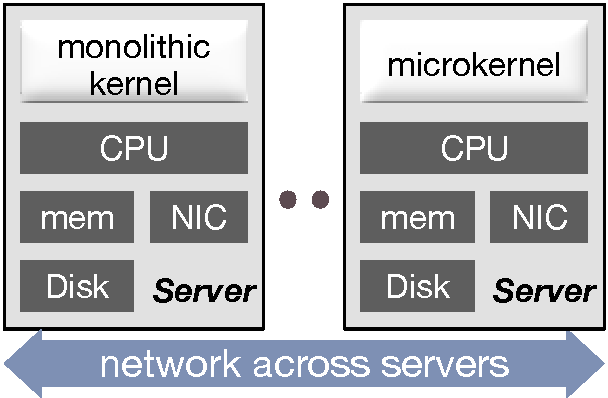
\includegraphics[width=1.7in]{lego/Figures/monolithic-arch.pdf}}
\caption[Monolithic OS.]{OSes Designed for Monolithic Servers.}
\label{fig-monolithic}
\end{center}
\end{subfigure}
\begin{minipage}{0.05in}
\hspace{0.05in}
\end{minipage}
\begin{subfigure}{1.8in}
\begin{center}
\centerline{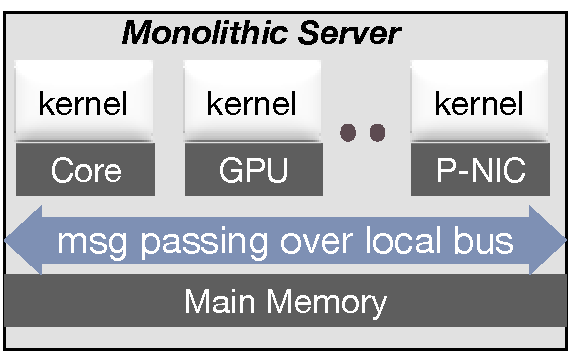
\includegraphics[width=1.8in]{lego/Figures/multikernel-arch.pdf}}
\caption[Multikernel Architecture.]{Multi-kernel Architecture. \small{P-NIC: programmable NIC.}}
\label{fig-multikernel}
\end{center}
\end{subfigure}
\begin{minipage}{0.05in}
\hspace{0.05in}
\end{minipage}
\begin{subfigure}{2.5in}
\begin{center}
\centerline{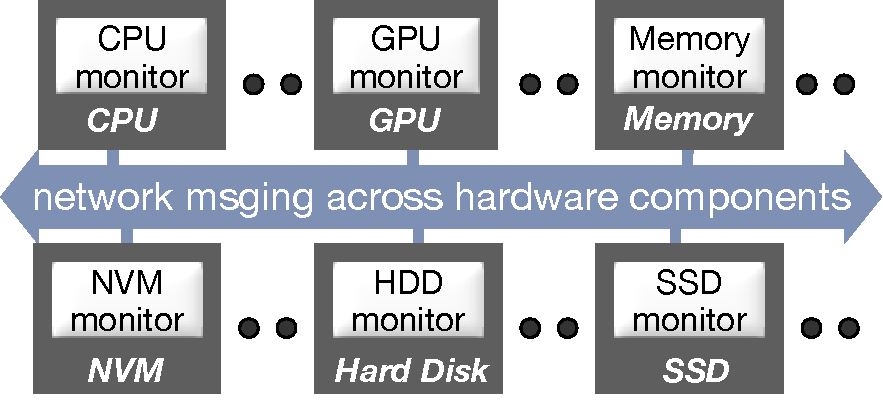
\includegraphics[width=2.6in]{lego/Figures/lego-arch.pdf}}
\caption[Splitkernel Architecture.]{Splitkernel Architecture.}
\label{fig-splitkernel}
\end{center}
\end{subfigure}
\caption[Operating System Architecture.]{Operating System Architecture.}
\end{figure*}
}

\ulinebfpara{Thread synchronization and data coherence.}
Threads and processes can share data even when they are not on the same \CN.
Similar to traditional concurrent programming, \sys\ threads can use synchronization primitives to build critical sections (\eg, with \syslock) 
and other semantics (\eg, flushing all requests with \fence).

An application can choose to cache data read from \Cliosysread\ at the \CN\ (\eg, by maintaining \texttt{local\_rbuf} in the code example).
Different processes sharing data in a \rspace\ can have their own cached copies at different \CN{}s.
Similar to ~\cite{Shan18-OSDI}, \sys\ does not make these cached copies coherent automatically and lets applications choose their own coherence
protocols.
%mechanisms and policies.
%Note that maintaining coherence when caching shared data is not handled by DVMA automatically. 
We made this deliberate decision because automatic cache coherence on every read/write would incur  high performance overhead with commodity Ethernet infrastructure
and application semantics could reduce this overhead.
%(\eg, by infrequent messaging).
%to let users decide on their coherence mechanism on top of \sys\ and to prevent the potential high network communication overhead.
%if threads cache shared data, there can be multiple locations of caches. 
%We do not make these caches coherent automatically, as it could cause high network communication overhead.
%Users can manage coherence on their own.
%Different users can share memory and can use \sys's synchronization primitives to achieve inter-user synchronization (\eg, using \tas\ to define critical section). 


\subsection{\sys\ Architecture}

In \sys\ (Figure~\ref{fig-arch}), \CN{}s are regular servers each equipped with a regular Ethernet NIC and connected to a top-of-rack (ToR) switch.
\MN{}s are our customized devices directly connected to a ToR switch.
%
Applications run at \CN{}s on top of our user-space library called {\em \syslib}.
%\syslib\ handles application requests in the user space.
It is in charge of request ordering, request retry, congestion, and incast control. 
%\syslib\ issues raw Ethernet requests directly to the NIC (bypassing kernel with zero memory copy, similar to DPDK~\cite{DPDK}). 
%Similar to DPDK~\cite{DPDK}, \syslib\ bypasses kernel and has zero memory copy capability.

By design, an \MN\ in \sys\ is a \sysboard\ consisting of an ASIC which runs the hardware logic for all data accesses (we call it the {\em fast path} and prototyped it with FPGA),
an ARM processor which runs software for handling metadata and control operations (\ie, the {\em slow path}),
and an FPGA which hosts application computation offloading (\ie, the {\em extend path}).
An incoming request arrives at the ASIC and travels through standard Ethernet physical and MAC layers 
and a Match-and-Action-Table (MAT) that decides which of the three paths the request should go to based on the request type.
If the request is a data access (fast path), it stays in the ASIC and goes through a hardware-based virtual memory system
that performs three tasks in the same pipeline: address translation, permission checking, and page fault handling (if any).
Afterward, the actual memory access is performed through the memory controller, and the response is formed and sent out through the network stack.
Metadata operations such as memory allocation are sent to the slow path. % and handled in software that runs on Linux at the ARM processor.
Finally, customized requests with %customized, high-level operations such as pointer chasing and 
offloaded computation are handled in the extend path.
%which executes the corresponding application offload.
%The offload itself could internally issue data and metadata operations to the fast and the slow paths.
%In the rest of the paper, we focus on the design of the fast and the slow paths and how they interact with each other.






\if 0
\subsection{Paper Scope And Potential Extensions}
\label{sec:scope}
%We made it real by building an open-source, distributed smart hardware-based disaggregated memory framework.
This paper focuses on the low-level systems problem of how to most efficiently build an \MN\ hardware device and to support it with \CN-side software. 
In real deployment, a single \sysboard\ is usually insufficient.
A distributed set of \sysboard\ would allow applications to allocate and access memory from multiple \MN{}s using a unified virtual memory interface. 
Systems like LegoOS~\cite{Shan18-OSDI} and Clover~\cite{Tsai20-ATC} have demonstrated how to build a distributed \MN\ platform.
For example, LegoOS uses a “two-level” approach, where a global controller manages the entire memory space at coarse granularity and each \MN\ manages its own memory at fine granularity (like how \sysboard\ does). Each \MN\ can be over-committed (\ie, allocating more virtual memory than its physical memory size), and when an \MN\ is under memory pressure, it migrates data to another \MN\ (coordinated by the global controller).
In addition, LegoOS leaves the handling of \MN\ failure to applications, since most data-center applications already have their own reliability mechanisms.
A similar mechanism could be used to extend \sys\ to a distributed system, and we leave it for future work.

Another potential extension to our current implementation of \sys\ is a transparent user interface.
By design, \sys’s APIs can be called by different layers: directly by applications as what we show in this paper, by a runtime like the AIFM runtime~\cite{AIFM}, or by the kernel/hardware at \CN\ like LegoOS' pComponent~\cite{Shan18-OSDI}. \sysboard\ doesn’t need any change to support any of these usages.
The latter two usages of \sysboard\ would result in a transparent interface and allow the use of unmodified user applications.
For example, for the last case, the \CN\ kernel or hardware captures misses in \CN’s local memory and then calls \sys’s APIs to fulfill the misses.
%(after porting \syslib\ to the kernel space or to hardware).

\fi


%\yizhou{Clio architecture shares a lot similarities with disaggregated storage systems such as fiber channel storage area network (FC SAN). The key difference is that Clio targets microsecond-level disaggregated memory system which poses stricter requirements on the system design.}


%\yizhou{
%1) I think we should explicitly say "By design, MN consists of ASIC, FPGA, and ARM parts.. In our impl, the ASIC part is using FPGA too." I get the motive behind it. The way it is described makes readers think this is the real stuff. 2) Similarly, the customized extend path does not really have to be FPGA as well. It could be ASIC too. In all, I suggest differentiate "by design" and "our impl".}

\if 0

\section{Hardware-Based Virtual Disaggregated Memory}
\label{sec:vdm}

We advocate for a new approach for memory disaggregation:
a hardware-based ``smart'' virtual disaggregated memory system.
Specifically, this approach encorporates the following design principles.
%We believe that disaggregated memory should be managed at the memory side behind a per-client virtual memory abstraction, 
%but without the reliance on a host server and with the support for computation offloading.
%With a per-client virtual memory abstraction, 
%application-level programs and low-level systems like databases and JVM can all sit on \sys\ with each of them properly isolated,
%and the physical location of disaggregated memory can be transparent and thus non-contiguous and moved around.
%By building a hardware-based ``smart'' virtual disaggregated memory system,
%we can achieve low-latency performance, scalability, efficient memory utilization, low cost, and ease of management,
%as what the rest of this paper will show.
%Below are the principles that guide the design of \sys.

\boldpara{Managing memory at \MN{}s and exposing a per-client virtual memory abstraction.}
We manage disaggregated memory entirely within a disaggregated memory pool by building a virtual memory system at each \MN.
By encapsulating management in the disaggregated memory pool and allowing client applications to
access it as a black box,
we can achieve independent, transparent resource pool management,
which is a key reason behind industry's wide adoption of storage disaggregation~\cite{FACEBOOK-BRYCECANYON,FB1,SnowFlake-NSDI20,Ali-SinglesDay}. %why storage disaggregation has become the recent industry norm;
It also avoids the network communication overhead incurred in solutions that handle some or all management tasks at \CN{}s.

We choose to expose a {\em per-client virtual memory} abstraction,
where each client has an isolated space that it can access with virtual memory addresses at byte granularity.
%\textbf{Q1)} \textit{what abstraction disaggregated memory exposes}?
%Disaggregated memory should expose an abstraction that is versatile enough to support many different uses.
%One such abstraction is {\em per-client virtual memory},
Just like the classical virtual memory abstraction, this abstraction is low-level and generic enough to support many applications
and high-level enough to protect and hide raw memory. 
%This abstraction inherits the versatility and transparency benefits of the classical virtual memory abstraction. %process address spaces:
%1) application-level programs and low-level systems like databases and JVM can all sit on the same abstraction
%with each of them properly isolated,
%and 2) the physical location of disaggregated memory can be transparent and thus non-contiguous and moved around.
%The abstraction we believe to be the best fit for memory disaggregation is a virtual memory interface that is facing client processes running at \CN{}s.
%With this abstraction, disaggregated memory can be managed at \MN{}s, which is more efficient and flexible than at \CN{}s (\S\ref{sec:intro} and \S\ref{sec:pdm}).
%It is worth noticing that %\sys\ is a versatile system that can either 
For example, memory disaggregation solutions that operate below the application level,
\eg, language runtime~\cite{Semeru}, data-structure library~\cite{AIFM}, swap system~\cite{InfiniSwap,FastSwap}, %\fixme{anything else?},
can sit on top of \sys. % and are orthogonal to our work. 
They can be ported to \sys\ by replacing their RDMA-/messaging-based abstraction to \sys's virtual memory abstraction. % (Figure~\ref{fig-usage} U3).

\boldpara{Building a virtual memory system in hardware.}
We demonstrate that \MN{}s can be built as standalone hardware devices without a server box,
as its benefits outweigh the complexity of hardware development.
Building \MN\ as a single hardware device avoids the monetary cost of a whole server box and the energy cost of a power-hungry CPU.
It also avoids the performance overhead of NIC talking to the host server for handling virtual memory tasks like page fault handling.
Moreover, a hardware implementation could allow greater parallelism and customized pipelines
that is crucial in supporting disaggregate memory's scalability goals (TB-level memory, thousands of clients)
and in meeting today's and future high-speed network line rate~\cite{TONIC}.
%Today's disaggregated memory systems unfortunately have a strong reliance on host CPU, MMU, and OS
%for running a virtual memory system, even though these systems themselves do not necessarily need to run anything at the host server.
%The solution is obvious but never carried out before: building the virtual memory system in \MN\ hardware.

\boldpara{Designing a network layer that exploits memory disaggregation's unique features.}
We improve network communication performance and reduce its costs by 
exploiting the unique nature of memory disaggregation. % to co-design a new network layer.
%Unfortunately, existing disaggregated memory systems lose this optimization opportunity by sitting on RDMA or TCP.
Unlike general-purpose network solutions such as TCP and RDMA that have the same design for all endpoints (\ie, symmetric),
the network system for disaggregated memory can be {\em asymmetric}, as \CN{}s are always the request initiator and \MN{}s only respond to requests.
%RDMA and TCP have two fundamental features that make them unfit for memory disaggregation:
%1) they have the same design for all endpoints (\ie, symmetric),
%while memory disaggregation are asymmetric in nature (\CN{}s are always the request initiator and \MN{}s only respond to requests);
Moreover, not all memory operations require strict ordering.
Thus, we can relax network layer's reliability guarantees (\eg, allowing packet reordering)
and enforce (weaker) orderings at the memory operation level.
%2) their reliable transports are connection-based and follow strict packet ordering.
%These features result in scalability bottlenecks and added hardware complexity.
%However, as we will show in \S\ref{sec:network}, neither are required if we can customize the network layer for the client-facing virtual memory model.

\boldpara{Supporting computation offloading with a unified virtual memory view.}
The network communication between \CN{}s and \MN{}s is the major cause of disaggregated memory's performance overhead.
To reduce this overhead, applications should be able to offload their less computation-intensive tasks to \MN{}s.
\sys\ offers a unified virtual memory view for application computation at both \CN\ and \MN.
%and offloads running at \MN{}s cannot have a coherent memory view with computation running at \CN{}s.
Furthermore, running offloaded computation in hardware is a desired option, %reduces \MN{}'s energy cost 
as it could achieve more parallelism and performance customization while avoiding CPU energy cost.
\sys\ allows offloads that run in hardware to use the \sys\ virtual memory interface in the same way as how software runs on \sys.
%However, %a major obstacle of hardware-based offloading currently is 
%it is hard to offload computation to \MN\ hardware today,
%largely because there is no good system support for offloads to use (virtualized) memory
%We build an offloading framework that offers a unified virtual memory view for application computation at both \%CN\ and \MN.
%applications should be able to easily and safely offload their less computation-intensive tasks to \MN{}s.




\section{Hardware Active Disaggregated Memory}
\label{sec:phdm}

%This section gives an overview of the \phdm\ model, 
%its benefits, and its use cases.

%\subsection{\phdm\ Overview}
%\label{sec:phdmoverview}

\phdm\ has a server-based compute pool that runs applications
and a separate memory pool that consists of network-attached hardware memory devices.
%\phdm\ has a distributed, network-attached memory pool 
%that is separated from the compute pool.
%\phdm\ manages memory at the remote memory pool.
%and runs applications at the compute pool.
An application process running at a \CN{} can use memory from any \MN{},
and an \MN{} can host data for many applications running on different \CN{}s.
%With this design of disaggregated and distributed memory services,
Thus, \phdm\ delivers independent management and scaling of memory and compute pools 
and efficient memory resource utilization.
%Doing so reduces network RTTs and makes management tasks such as configuration, upgrade, and failure handling easy
%with no or little disturbance to \CN{}s.

An \phdm\ system manages and virtualizes physical memory at \MN{}s
and offers one or more {\em distributed memory services}.
\phdm\ provides a protected, client-centric virtual memory abstraction 
and potentially more higher-level memory service interfaces.
Applications running at \CN{}s can directly and safely use these interfaces to access remote memory. % and be protected from each other.
%These services have a client-centric view, providing interfaces that can directly and easily be used by clients 
%and offering proper protection across different applications.
%It provides high-level memory services and
% can support new types of applications that require large memory space, 
%inter-node memory sharing, or fast data storage.
%Section~\ref{sec:usecases} gives several examples of \phdm\ memory services.

\phdm\ executes all performance-critical tasks on hardware at \MN{}s,
%As explained in \S\ref{sec:disaggregation}, 
%With fast increasing datacenter network bandwidth, \MN{}s need to be able to serve large amounts of 
%requests concurrently to deliver {\em network line-rate} performance.
%Running software in many-core CPU could potentially meet the performance requirement but comes with high monetary and energy cost,
%while running software in low-energy ``wimpy'' cores cannot keep up with high network line rate.
%as handling memory requests in hardware is critical in meeting 
as doing so can meet the performance, scalability, and cost goals of remote memory systems.
With varying application needs in today's datacenters,
disaggregated memory systems should be flexible enough to provide different services and interfaces.
Thus, in our proposed \phdm\ model, the remote memory layer is {\em reconfigurable}.
%We further propose to implement \phdm's memory services on programmable hardware
%to meet our target usage and deployment models:
Specifically, an \MN{} can be configured to offer different (sets of) memory services,
but once a cluster of \MN{}s are configured they are only reconfigured when 
there is a need to change, patch, or upgrade services.
This model is in line with Microsoft's FPGA deployment~\cite{Catapult}
and what we view as a good use of reconfigurable hardware in datacenters.

\if 0
Finally, we view \phdm\ as a general model that can have different hardware choices for \MN{}s,
as long as they incorporate some programmable hardware for performance-critical and non-fixed tasks in memory services
(\eg, a single FPGA, FPGA+SoC, ASIC+FPGA, or ASIC+FPGA+SoC).
Non-performance-critical tasks can run in software, and fixed functionalities can run in non-programmable hardware.
\fi


%\subsection{Use Cases}
%\label{sec:usecases}
Many types of applications can make use of \phdm.
%In some cases, applications could explicitly call APIs an \phdm\ service provides
%(and be aware of the disaggregated nature of their in-memory data).
%In other cases, they could transparently access an \phdm\ service without knowing the disaggregated or remote nature.
Below we give some examples. % on what services an \phdm\ system can provide and how applications can use them.
We implemented an instance of the first three types in this paper,
leaving the rest for future work.

\boldpara{Extended (semantic-rich) virtual memory.}
A basic service \phdm\ can provide is a remote virtual memory space that lets applications
store in-memory data (\eg, as extended, slower heaps).
%Similar to traditional process address spaces, each application process on each \CN{}
%can have their own remote address space that \phdm\ protects from other processes'.
In addition to simple, hardware-like virtual memory APIs such as reading and writing to a memory address, 
\phdm\ could provide higher-level APIs like synchronization primitives, pointer manipulation, 
vector and scatter-gather operations~\cite{Aguilera-FarMemory}.
Applications and language libraries can then build complex data structures like vectors 
and trees with these APIs.
%We implemented this extended virtual memory service in \sys.

\boldpara{In-memory and ephemeral storage.}
\phdm\ could offer in-memory storage services such as distributed key-value stores, databases, and file systems.
With \phdm, many storage operations (\eg, key-value pair lookup, SQL select) 
could be implemented in hardware at where the data is, offering enhanced performance. 
%In addition, built-in distributed support in \phdm\ could be used to offer high availability and failure resilience
%to the in-memory storage services.
\phdm\ is also a good fit for building ephemeral storage and storage caching that do not require failure resilience~\cite{SnowFlake-NSDI20,Pocket,fitzpatrick2004distributed}.
%We implemented a distributed key-value store in \sys\ with optional replication support.

\boldpara{Data sharing.}
Since multiple \CN{}s can access the same \MN{}s in \phdm,
\phdm\ could be used for data sharing and communication across \CN{}s.
This is especially useful for new datacenter services like serverless computing~\cite{Berkeley-Serverless},
which currently has no or poor support for managing states and inter-function communication.
With \phdm, serverless functions can run on \CN{}s and store states or communication messages in the disaggregated memory layer.
Similarly, \phdm\ can also be used for storing global states such as the parameter server in distributed machine learning systems.
%We implemented a multi-version data sharing service in \sys\
%that can be accessed by different \CN{}s concurrently.

\boldpara{Offloading data processing.}
\phdm\ is a good candidate for offloading data processing and data analytics. 
Data-intensive applications can offload computation that frequently access in-memory data together with 
these data to \MN{}s.
One such example is disaggregated Spark shuffle~\cite{Stuedi-ATC19}, where the shuffle
operation could be implemented in programmable hardware and the shuffle data could be 
stored in \MN{}s of \phdm.

\boldpara{Remote swap and remote disk.}
Legacy applications and libraries can also benefit from \phdm\ in a transparent way.
Two such examples are remote memory-based disk and remote swap~\cite{InfiniSwap}.
The OS at the \CN{}s can add a memory-based block device that sits in \phdm\
in a similar way as building the {\em ramdisk} module.
Applications can directly use this new device or use it as a swap space.

\boldpara{Disaggregated OS.}
Recently, there have been proposals to completely disaggregate memory from compute.
\lego~\cite{Shan18-OSDI} is such a proposal that organizes compute nodes as processors with no memory 
and \MN{}s as memory devices with no computation.
%While \lego\ currently only works on emulated hardware, it can build on \phdm\ to have a 
%real hardware solution.
\lego\ can build on \phdm\ by configuring \CN{}s as its compute nodes %(called {\em pComponent}s) 
and \MN{}s as its memory nodes. %(called {\em mComponent}s).


\fi
